% Generated by Sphinx.
\def\sphinxdocclass{report}
\documentclass[letterpaper,10pt,oneside]{sphinxmanual}
\usepackage[utf8]{inputenc}
\DeclareUnicodeCharacter{00A0}{\nobreakspace}
\usepackage{cmap}
\usepackage[T1]{fontenc}
\usepackage[english]{babel}
\usepackage{times}
\usepackage[Bjarne]{fncychap}
\usepackage{longtable}
\usepackage{sphinx}
\usepackage{multirow}


\title{FreeJournal Documentation}
\date{May 03, 2015}
\release{1.0}
\author{https://github.com/FreeJournal/}
\newcommand{\sphinxlogo}{}
\renewcommand{\releasename}{Release}
\makeindex

\makeatletter
\def\PYG@reset{\let\PYG@it=\relax \let\PYG@bf=\relax%
    \let\PYG@ul=\relax \let\PYG@tc=\relax%
    \let\PYG@bc=\relax \let\PYG@ff=\relax}
\def\PYG@tok#1{\csname PYG@tok@#1\endcsname}
\def\PYG@toks#1+{\ifx\relax#1\empty\else%
    \PYG@tok{#1}\expandafter\PYG@toks\fi}
\def\PYG@do#1{\PYG@bc{\PYG@tc{\PYG@ul{%
    \PYG@it{\PYG@bf{\PYG@ff{#1}}}}}}}
\def\PYG#1#2{\PYG@reset\PYG@toks#1+\relax+\PYG@do{#2}}

\expandafter\def\csname PYG@tok@gd\endcsname{\def\PYG@tc##1{\textcolor[rgb]{0.63,0.00,0.00}{##1}}}
\expandafter\def\csname PYG@tok@gu\endcsname{\let\PYG@bf=\textbf\def\PYG@tc##1{\textcolor[rgb]{0.50,0.00,0.50}{##1}}}
\expandafter\def\csname PYG@tok@gt\endcsname{\def\PYG@tc##1{\textcolor[rgb]{0.00,0.27,0.87}{##1}}}
\expandafter\def\csname PYG@tok@gs\endcsname{\let\PYG@bf=\textbf}
\expandafter\def\csname PYG@tok@gr\endcsname{\def\PYG@tc##1{\textcolor[rgb]{1.00,0.00,0.00}{##1}}}
\expandafter\def\csname PYG@tok@cm\endcsname{\let\PYG@it=\textit\def\PYG@tc##1{\textcolor[rgb]{0.25,0.50,0.56}{##1}}}
\expandafter\def\csname PYG@tok@vg\endcsname{\def\PYG@tc##1{\textcolor[rgb]{0.73,0.38,0.84}{##1}}}
\expandafter\def\csname PYG@tok@m\endcsname{\def\PYG@tc##1{\textcolor[rgb]{0.13,0.50,0.31}{##1}}}
\expandafter\def\csname PYG@tok@mh\endcsname{\def\PYG@tc##1{\textcolor[rgb]{0.13,0.50,0.31}{##1}}}
\expandafter\def\csname PYG@tok@cs\endcsname{\def\PYG@tc##1{\textcolor[rgb]{0.25,0.50,0.56}{##1}}\def\PYG@bc##1{\setlength{\fboxsep}{0pt}\colorbox[rgb]{1.00,0.94,0.94}{\strut ##1}}}
\expandafter\def\csname PYG@tok@ge\endcsname{\let\PYG@it=\textit}
\expandafter\def\csname PYG@tok@vc\endcsname{\def\PYG@tc##1{\textcolor[rgb]{0.73,0.38,0.84}{##1}}}
\expandafter\def\csname PYG@tok@il\endcsname{\def\PYG@tc##1{\textcolor[rgb]{0.13,0.50,0.31}{##1}}}
\expandafter\def\csname PYG@tok@go\endcsname{\def\PYG@tc##1{\textcolor[rgb]{0.20,0.20,0.20}{##1}}}
\expandafter\def\csname PYG@tok@cp\endcsname{\def\PYG@tc##1{\textcolor[rgb]{0.00,0.44,0.13}{##1}}}
\expandafter\def\csname PYG@tok@gi\endcsname{\def\PYG@tc##1{\textcolor[rgb]{0.00,0.63,0.00}{##1}}}
\expandafter\def\csname PYG@tok@gh\endcsname{\let\PYG@bf=\textbf\def\PYG@tc##1{\textcolor[rgb]{0.00,0.00,0.50}{##1}}}
\expandafter\def\csname PYG@tok@ni\endcsname{\let\PYG@bf=\textbf\def\PYG@tc##1{\textcolor[rgb]{0.84,0.33,0.22}{##1}}}
\expandafter\def\csname PYG@tok@nl\endcsname{\let\PYG@bf=\textbf\def\PYG@tc##1{\textcolor[rgb]{0.00,0.13,0.44}{##1}}}
\expandafter\def\csname PYG@tok@nn\endcsname{\let\PYG@bf=\textbf\def\PYG@tc##1{\textcolor[rgb]{0.05,0.52,0.71}{##1}}}
\expandafter\def\csname PYG@tok@no\endcsname{\def\PYG@tc##1{\textcolor[rgb]{0.38,0.68,0.84}{##1}}}
\expandafter\def\csname PYG@tok@na\endcsname{\def\PYG@tc##1{\textcolor[rgb]{0.25,0.44,0.63}{##1}}}
\expandafter\def\csname PYG@tok@nb\endcsname{\def\PYG@tc##1{\textcolor[rgb]{0.00,0.44,0.13}{##1}}}
\expandafter\def\csname PYG@tok@nc\endcsname{\let\PYG@bf=\textbf\def\PYG@tc##1{\textcolor[rgb]{0.05,0.52,0.71}{##1}}}
\expandafter\def\csname PYG@tok@nd\endcsname{\let\PYG@bf=\textbf\def\PYG@tc##1{\textcolor[rgb]{0.33,0.33,0.33}{##1}}}
\expandafter\def\csname PYG@tok@ne\endcsname{\def\PYG@tc##1{\textcolor[rgb]{0.00,0.44,0.13}{##1}}}
\expandafter\def\csname PYG@tok@nf\endcsname{\def\PYG@tc##1{\textcolor[rgb]{0.02,0.16,0.49}{##1}}}
\expandafter\def\csname PYG@tok@si\endcsname{\let\PYG@it=\textit\def\PYG@tc##1{\textcolor[rgb]{0.44,0.63,0.82}{##1}}}
\expandafter\def\csname PYG@tok@s2\endcsname{\def\PYG@tc##1{\textcolor[rgb]{0.25,0.44,0.63}{##1}}}
\expandafter\def\csname PYG@tok@vi\endcsname{\def\PYG@tc##1{\textcolor[rgb]{0.73,0.38,0.84}{##1}}}
\expandafter\def\csname PYG@tok@nt\endcsname{\let\PYG@bf=\textbf\def\PYG@tc##1{\textcolor[rgb]{0.02,0.16,0.45}{##1}}}
\expandafter\def\csname PYG@tok@nv\endcsname{\def\PYG@tc##1{\textcolor[rgb]{0.73,0.38,0.84}{##1}}}
\expandafter\def\csname PYG@tok@s1\endcsname{\def\PYG@tc##1{\textcolor[rgb]{0.25,0.44,0.63}{##1}}}
\expandafter\def\csname PYG@tok@gp\endcsname{\let\PYG@bf=\textbf\def\PYG@tc##1{\textcolor[rgb]{0.78,0.36,0.04}{##1}}}
\expandafter\def\csname PYG@tok@sh\endcsname{\def\PYG@tc##1{\textcolor[rgb]{0.25,0.44,0.63}{##1}}}
\expandafter\def\csname PYG@tok@ow\endcsname{\let\PYG@bf=\textbf\def\PYG@tc##1{\textcolor[rgb]{0.00,0.44,0.13}{##1}}}
\expandafter\def\csname PYG@tok@sx\endcsname{\def\PYG@tc##1{\textcolor[rgb]{0.78,0.36,0.04}{##1}}}
\expandafter\def\csname PYG@tok@bp\endcsname{\def\PYG@tc##1{\textcolor[rgb]{0.00,0.44,0.13}{##1}}}
\expandafter\def\csname PYG@tok@c1\endcsname{\let\PYG@it=\textit\def\PYG@tc##1{\textcolor[rgb]{0.25,0.50,0.56}{##1}}}
\expandafter\def\csname PYG@tok@kc\endcsname{\let\PYG@bf=\textbf\def\PYG@tc##1{\textcolor[rgb]{0.00,0.44,0.13}{##1}}}
\expandafter\def\csname PYG@tok@c\endcsname{\let\PYG@it=\textit\def\PYG@tc##1{\textcolor[rgb]{0.25,0.50,0.56}{##1}}}
\expandafter\def\csname PYG@tok@mf\endcsname{\def\PYG@tc##1{\textcolor[rgb]{0.13,0.50,0.31}{##1}}}
\expandafter\def\csname PYG@tok@err\endcsname{\def\PYG@bc##1{\setlength{\fboxsep}{0pt}\fcolorbox[rgb]{1.00,0.00,0.00}{1,1,1}{\strut ##1}}}
\expandafter\def\csname PYG@tok@mb\endcsname{\def\PYG@tc##1{\textcolor[rgb]{0.13,0.50,0.31}{##1}}}
\expandafter\def\csname PYG@tok@ss\endcsname{\def\PYG@tc##1{\textcolor[rgb]{0.32,0.47,0.09}{##1}}}
\expandafter\def\csname PYG@tok@sr\endcsname{\def\PYG@tc##1{\textcolor[rgb]{0.14,0.33,0.53}{##1}}}
\expandafter\def\csname PYG@tok@mo\endcsname{\def\PYG@tc##1{\textcolor[rgb]{0.13,0.50,0.31}{##1}}}
\expandafter\def\csname PYG@tok@kd\endcsname{\let\PYG@bf=\textbf\def\PYG@tc##1{\textcolor[rgb]{0.00,0.44,0.13}{##1}}}
\expandafter\def\csname PYG@tok@mi\endcsname{\def\PYG@tc##1{\textcolor[rgb]{0.13,0.50,0.31}{##1}}}
\expandafter\def\csname PYG@tok@kn\endcsname{\let\PYG@bf=\textbf\def\PYG@tc##1{\textcolor[rgb]{0.00,0.44,0.13}{##1}}}
\expandafter\def\csname PYG@tok@o\endcsname{\def\PYG@tc##1{\textcolor[rgb]{0.40,0.40,0.40}{##1}}}
\expandafter\def\csname PYG@tok@kr\endcsname{\let\PYG@bf=\textbf\def\PYG@tc##1{\textcolor[rgb]{0.00,0.44,0.13}{##1}}}
\expandafter\def\csname PYG@tok@s\endcsname{\def\PYG@tc##1{\textcolor[rgb]{0.25,0.44,0.63}{##1}}}
\expandafter\def\csname PYG@tok@kp\endcsname{\def\PYG@tc##1{\textcolor[rgb]{0.00,0.44,0.13}{##1}}}
\expandafter\def\csname PYG@tok@w\endcsname{\def\PYG@tc##1{\textcolor[rgb]{0.73,0.73,0.73}{##1}}}
\expandafter\def\csname PYG@tok@kt\endcsname{\def\PYG@tc##1{\textcolor[rgb]{0.56,0.13,0.00}{##1}}}
\expandafter\def\csname PYG@tok@sc\endcsname{\def\PYG@tc##1{\textcolor[rgb]{0.25,0.44,0.63}{##1}}}
\expandafter\def\csname PYG@tok@sb\endcsname{\def\PYG@tc##1{\textcolor[rgb]{0.25,0.44,0.63}{##1}}}
\expandafter\def\csname PYG@tok@k\endcsname{\let\PYG@bf=\textbf\def\PYG@tc##1{\textcolor[rgb]{0.00,0.44,0.13}{##1}}}
\expandafter\def\csname PYG@tok@se\endcsname{\let\PYG@bf=\textbf\def\PYG@tc##1{\textcolor[rgb]{0.25,0.44,0.63}{##1}}}
\expandafter\def\csname PYG@tok@sd\endcsname{\let\PYG@it=\textit\def\PYG@tc##1{\textcolor[rgb]{0.25,0.44,0.63}{##1}}}

\def\PYGZbs{\char`\\}
\def\PYGZus{\char`\_}
\def\PYGZob{\char`\{}
\def\PYGZcb{\char`\}}
\def\PYGZca{\char`\^}
\def\PYGZam{\char`\&}
\def\PYGZlt{\char`\<}
\def\PYGZgt{\char`\>}
\def\PYGZsh{\char`\#}
\def\PYGZpc{\char`\%}
\def\PYGZdl{\char`\$}
\def\PYGZhy{\char`\-}
\def\PYGZsq{\char`\'}
\def\PYGZdq{\char`\"}
\def\PYGZti{\char`\~}
% for compatibility with earlier versions
\def\PYGZat{@}
\def\PYGZlb{[}
\def\PYGZrb{]}
\makeatother

\renewcommand\PYGZsq{\textquotesingle}

\begin{document}

\maketitle
\tableofcontents

\chapter{Design and Goals}
\label{design:welcome-to-freejournal-s-documentation}\label{design::doc}\label{design:design-and-goals}

\href{http://freejournal.org/}{freejournal} is a system for securely publishing documents to the public,
releasing them to minimize risk to the publisher while making the documents difficult to censor, supress, or
alter once published.  FreeJournal is designed to replace organizations like
\href{https://wikileaks.org/}{WikiLeaks} with a peer-to-peer, decentralized network that allows any
user to publish any content they deem useful or interesting.

FreeJournal runs on the \href{https://bitmessage.org/}{Bitmessage}, \href{https://freenetproject.org/}{Freenet},
and \href{https://bitcoin.org/}{Bitcoin} networks, and its source is hosted on
\href{https://github.com/FreeJournal/freejournal}{Github}.  Please report any issues, bugs, or unclear
documentation you encounter there.



freejournal is a document publication system intended to allow the public release of documents in a way that is resistant to
suppression or censorship.

Whistleblowers, journalists, and others need a way to anonymously publish documents to a public or private audience of their
choosing.  Currently, they do so through complex anonymity software restricted to developers and cryptography experts, or
through third-party institutions prone to internal politics and editorializing like Wikileaks.  Many other users sharing less
sensitive content defer the storage and management of their information to third-party services, like LiveJournal, imgur, or any
number of other content hosting companies.  freejournal is a protocol and accompanying user-friendly front end application
designed to assist in the anonymous and uncensorable release of documents to a public audience in a cryptographically secure
manner, without requiring trust in any third party services.  FreeJournal can greatly improve freedom of information worldwide
by allowing for open, anonymous releases of documents not vulnerable to manipulation by any third party.


\section{Participants/Actors}
There are several roles an individual can adopt when interacting with the FreeJournal software:
\label{design:participants-actors}


\subsection{Document Viewers}
\label{design:document-viewers}
Document viewers are individual users who are interested in browsing a document.  This could be either because they were
told to or linked to view the document, or simply out of curiosity regarding what new documents are being published.
Such a user will have two choices: they can run their own version of the freejournal software, hosting the web interface
locally on their machine and accessing it through any browser at \emph{localhost}.

Alternatively, these users can simply visit the web interface hosted by a ``node'' they trust.  This ``node'' is hosted by
another user or organization, and can be accessed through HTTP or any protocol supporting HTTP (like Tor, I2P, cjdns, etc.)
This will likely be the common usage pattern for most users, who desire convenience over security and who are willing to
trust a node run by a reputable organization or party to serve them accurate content.


\subsection{Document Publishers}
\label{design:document-publishers}
Document publishers are those wishing to publicly release documents in a way immune to third-party manipulation or censorship.
These users often value their security and anonymity above convenience, and often wish to conceal or disguise their real
identities to the public.  For these users, we will provide a \textbf{document uploader} application.  This application will work
in a virtual machine that communicates to the Internet exclusively through the Tor anonymity network, providing the maximum
possible isolation for these users from network traffic inspection attacks.


\subsection{Nodes / Infrastructure Providers}
\label{design:nodes-infrastructure-providers}
In such a network, it is critical to have the infrastructure to host and serve documents to new users interested in downloading
them.  While traditional services handle this with a centralized database, freejournal is a p2p system and thus makes use of
nodes.  Nodes are instances of the freejournal project which host documents uploaded to the network and relay them to other
users.  Nodes also are responsible for the upkeep of the network, as well as its synchronization that allows all users to
obtain the documents they are interested in.

Nodes will be run by users who are interested in supporting free speech, similar to the users running Tor relays, Freenet nodes,
or other peer-to-peer anonymity network nodes.  These users will donate disk-space, often on high powered servers, to cache
and redistribute freejournal documents.  Nodes will also often be interested in controlling the content they mirror, removing
offensive and illegal content from their machines as necessary to avoid violating laws in their jurisdictions.


\section{Project Motivation}
\label{design:project-motivation}
The need for open document publishing and whistle blowing in society is a well established philosophical argument that hinges on
the fundamental right to share and exchange information freely and without censorship.  The famous \href{https://en.wikipedia.org/wiki/Panopticon}{panopticon experiment} imagines a society in which the constant surveillance of all its members leads to a
crippling of intellectual debate, arguing for a strong need for open information sharing.  Despite this, it remains
prohibitively difficult to share such information, requiring advanced technical precautions to do so with any level of
anonymity.  We seek to provide an open, safe and global public space for the release and discussion of any sort of documents,
strongly resistant to being censored or attacked by any third party or group.  In doing so, our motivation is to foster
transparency and debate on controversial primary source material.

Previously, the role of mediating document release to the public fell to journalistic organizations, both corporate (New York
Times, The Guardian, etc.) and community-based (WikiLeaks, OpenSecrets, etc.)  An organizational approach to this fundamental
problem, however, is fatally and deeply flawed.  Publishers of documents must trust this third-party to accurately and wholly
publish their information.  Furthermore, publishers must coordinate the transfer of this information, often involving advanced
technical precautions.  The involvement of third parties in any system required to provide strong security guarantees is
considered by many security experts to be a security hole, \href{http://szabo.best.vwh.net/ttps.html}{unacceptable in a system for open document release}.

The freejournal project attempts to bridge this gap by providing a system for public document release that is not controlled
by any particular third party, and is open to all users in a document-agnostic fashion.


\section{Terminology}
\label{design:terminology}
\textbf{Documents} : Documents are files that are leaked to the FreeJournal network.  Documents have an associated name, description,
timestamp, and file that can be viewed.

\textbf{Collections} : Collections are groups of documents, published together by the same user.  Collections can be updated (documents
added, removed), timestamped, and browsed together.  Nodes can blacklist or whitelist which connections they wish to mirror.


\section{Components}
\label{design:components}
The FreeJournal is made up of the following several components attempting to achieve the aforementioned goals:


\subsection{Backend/Library}
\label{design:backend-library}
The backend/library of freejournal provides an abstraction of the FreeJournal network into Python objects, powering all other
interfaces described below.  The backend/library includes a relational database used for caching incoming network objects.


\subsection{Command-Line Interface}
\label{design:command-line-interface}
The command line interface is designed to allow node operators and power users to interact with the network.  It will support
all essential network tasks, including document/collection maintenance, publication, and retrieval.  It will also provide an
easy way to launch the web interface, install dependencies, and run the uploader application.


\subsection{Web Interface}
\label{design:web-interface}
The web interface is designed to allow users to view, timestamp, and otherwise interact with uploaded documents and collections
to the network.  The web interface should be familiar to users of other web services, and provide an abstraction of the underlying
FreeJournal peer-to-peer network for users.  The web interface should not support uploading for security purposes.


\subsection{Uploader Application}
\label{design:uploader-application}
The uploader application is designed to provide securit to document uploaders, allowing for a relatively easy to use interface
that ensures the anonymity and integrity of the documents being submitted are protected.  The uploader application will eventually
be packaged in a virtual machine supporting the Tor anonymity network.


\section{High-Level Goals}
\label{design:high-level-goals}
This project aims to accomplish the following core goals, differentiating us from currently available projects:

\textbf{User friendliness} - Many of the other applications targeted at the secure and confidential release of documents require high
levels of technical proficiency reserved for advanced technical actors.  We aim to allow the ordinary user to engage with
FreeJournal, with a clear and simple user interface familiar to users of little technical proficiency.

\textbf{Modular design} - By designing both a library to support our document release protocol and a separate user interface for
users to easily add and view documents, we allow for a variety of front-end implementations, from desktop apps and virtual
machines to webapps.  Building an open protocol on top of the already existing open Bitmessage protocol ensures that future
developers can easily build applications to integrate with FreeJournal.

\textbf{Deniability} - One of the central concerns of publishers of controversial material is their ability to be identified.  We aim
to provide automatic steps to remove identifying information from source documents, and deniability of communications over the
wire such that an eavesdropping attacker would be unable to ascertain whether a user of the system did or did not publish any
documents (or indeed use the system at all).

\textbf{Trust} - In order to allow for curation and verification of source material usually only possible through a traditional,
top-down editorial process, we will provide a platform for public discourse and analysis of the documents, as well as a system
for users to rank and promote trustworthy documents to other users of the system.  We will do so by allowing users to support
document publishers through peer to peer tokens like Bitcoin, providing both a reward for quality content and a ranking system
that would be expensive for an adversary to attack.

\textbf{Transparency} - We aim to ensure that every aspect of our system is open in both design and implementation.  We plan on using
unique cryptographic properties extending those used in Bitcoin and the Bitmessage protocol to provide clear and auditable
information to the public about which documents were published together and when certain documents were published.  Through such
an open system, we will provide an auditable process for document publishers, who can determine exactly the steps their document
will take through the publication process (unlike in shadowy and closed organizations like newspapers).

\textbf{Inclusiveness} - By the design of the network, its participation will be open to all.  We aim to require no fees in order to
publish or read documents, and to provide easy tools that can be used by users of all technical proficiencies.  We also plan on
providing a protocol that is resistant to censorship or manipulation, allowing all potential users to engage with the system
regardless of their motivation or personal views or character.

\textbf{Confidentiality} - One key usecase for FreeJournal is the ability for existing journalists to gather documents.  To address
this usecase, we will allow groups of documents to be published only to private users or groups, so that existing journalist
outlets need only post their FreeJournal account to have private leaks disseminated directly through them via this public
protocol.  We will protect the confidentiality of such documents by encryption.  Furthermore, we will enforce pseudonymity as a
requirement, ensuring that FreeJournal accounts are unlinkable to real-world identities.

\textbf{Integrity and Availability} - By building on the Bitmessage platform, we are leveraging a global peer-to-peer network that is
designed to be robust and immune to censorship or takedown attempts.  We use the blockchain data structure to protect published
documents and ensure they reach their intended audience without censorship.  We use the distributed node system already
available in Bitmessage to ensure that FreeJournal cannot be taken down by targeting a specific organization or set of servers,
as long as there are nodes in the network.  We leverage cryptography heavily to authenticate groups of documents and users
publishing these documents, and will provide methods to check that users running the FreeJournal software are running an
unmodified version with no tampering or backdoors.

\textbf{Fine-grained control} - We believe that any protocol addressing these issues must be fundamentally document-agnostic, and
cannot inherently censor or discriminate against any particular class of documents.  However, as some documents uploaded may be
illegal in certain jurisdictions or controversial for other reasons, we also believe it is the choice of each individual node
operator to be able to either whitelist or blacklist the items they store or relay, providing them fine-grained control of the
traffic flowing through their machine and allowing them to stop relaying items passing through their node at any time.  Because
the data structures required to maintain the integrity of the network do not depend on our individual nodes providing all
content, any exclusions on the part of a node will be clear to any user querying that node, maintaining the transparency and
availability requirements previously mentioned.


\section{Comparison to Similar Software}
\label{design:comparison-to-similar-software}
\textbf{Bitmessage} - \href{http://bitmessage.org}{Bitmessage} is a peer-to-peer communications protocol intended to be distributed,
peer-to-peer, pseudonymous, and cryptographically secure.  One of the use cases outlined initially during the design of the
BitMessage system was the leaking or \href{https://bitmessage.org/forum/index.php?topic=3.0}{release of documents}.  However,
BitMessage only provides utility to message other users or groups, lacking utilities to evaluate and rank documents, provide for
lasting public archival, or provide for public discourse and evaluation.  The lack of these features means a third-party
journalistic entity like WikiLeaks or a traditional newspaper must receive these documents, opening up potential opportunities
for the introduction of bias and violation of source integrity.  Furthermore, BitMessage has key technical problems rendering it
unsuitable for distributed document distribution - messages in the network often have a short lifespan, sometimes only lasting
days, and communication channels have not been shown to stand up against serious attack.  Lastly, BitMessage has no frontend
providing for clear user explanation and interaction, rendering it unsuitable for all but the most technical users. In this
regard, we believe BitMessage represents only a component of the ideal system we describe in our Motivation section.

\textbf{Wikileaks} - The most similar complete solution to what we are proposing is the journalistic organization \href{http://wikileaks.org/}{Wikileaks}, an organization allowing users to view and submit documents publicliy through the Internet and
promising for minimal discrimination.  Despite this, several high-profile failings of Wikileaks make it a poor choice for such
purposes.  In the past, organizational insiders have destroyed documents and otherwise compromised the integrity of the
organization (\href{https://darkhorsenet.wordpress.com/2013/01/08/daniel-domscheit-berg-the-man-who-sold-out-wikileaks-2/}{https://darkhorsenet.wordpress.com/2013/01/08/daniel-domscheit-berg-the-man-who-sold-out-wikileaks-2/}).
Furthermore, like any organization, Wikileaks’ key members are vulnerable to attack by powerful entities, weakening the
organization and proving it to not be resilient.  Other leaking organizations like OpenSecrets attempt to maintain transparency
through organizational practices, however we believe this is far from ideal.  If these organizations could be replaced with
peer-to-peer protocols allowing for document and information exchange, the guarantees provided to the document publishers become
well-defined and mathematically rigorous, guaranteeing full control of their published documents.

\textbf{Freenet} - \href{https://freenetproject.org/}{Freenet} is a distributed data store specifically designed for the publication of
files and documents specifically intended and targetted at the publication of controversial information.  In this regard,
Freenet is the most similar project to our intended design in its ambitions and design.  Freenet is based on a complex system of
encrypted node-based routing and distributed hash tables which provide excellent anonymity and deniability guarantees.  Unlike
our proposal, however, Freenet allows for minimal transparency and inclusiveness by making it difficult to achieve low-latency
interaction between large numbers of users.  Freenet is also unable to provide the integrity guarantees available to the Bitcoin
blockchain, in which strict timestamp guarantees resistant to even targeted adversarial attacks are provided.  Furthermore,
Freenet is extremely slow, requiring several hours for initial synchronization and often minutes for file downloads,
unacceptable for the real-time experience users expect from web applications today.  Freenet is far from user friendly and lacks
good front-end software, and lastly inherently lacks the ability to create a meaningful crowd-ranking system able to filter
content for quality and accuracy without the introduction of an additional protocol (due to its design, strict anonymity, and
inclusiveness).  On the other hand, Freenet is a mature project that may be used in the backend of our system if we find the
storage problem too difficult to solve with Bitmessage, sacrificing speed for project maturity.

\textbf{Tor/I2P} - We will briefly mention these projects for their ability to provide low-latency access to web services
anonymously.  These are not really comparable to our proposed system as they only provide a means of passing messages and not a
fully integrated platform for discussion and open publication for information.  However, both projects provide mature,
well-tested, and strong anonymity guarantees that make them ideal for users using our system who wish to add an extra layer of
anonymity.  We will aim to support the use of such software to offer our users an existing and secure way to interact with our
system without the need for our own encrypted routing scheme.


\chapter{Development Process}
\label{process:development-process}\label{process::doc}

\section{Git Standards}
\label{process:git-standards}
Generally, we followed Git model described in {[}this
document{]}(\href{http://nvie.com/posts/a-successful-git-branching-model/}{http://nvie.com/posts/a-successful-git-branching-model/}). Here are some of the key concepts.


\subsection{The \emph{develop} branch}
\label{process:the-develop-branch}
\emph{develop} was considered the go-to branch to start work. All changes that people make eventually get
merged into develop.


\subsection{Feature branches}
\label{process:feature-branches}
When working on an issue, we created new branches off of \emph{develop} and named it something relevant to the feature
that was being implemented. Once done working on the issue, we mark it with the \emph{needs-review} label.
After another team member reviews it, it can be merged into \emph{develop} by the branch maintainer for that iteration.


\subsection{The \emph{master} branch}
\label{process:the-master-branch}
The master branch should only have finished, bug-free code that represents a complete released version. At the
end of every sprint, we tag a commit on \emph{master} to represent the work completed for that iteration.
Unlike the model described in the blog post, we will not use release or hotfix branches as they're overkill
for a project of this size.


\subsection{Some helpful commands}
\label{process:some-helpful-commands}
Start a new feature branch:

\code{{}`
\$ git checkout develop
\$ git checkout -b myfeature
{}`}

Merge a feature branch into \emph{develop}:

\code{{}`
\$ git checkout develop
\$ git merge -{-}no-ff myfeature
{}`}

Update \emph{master} and tag a release:

\code{{}`
\$ git checkout master
\$ git merge -{-}no-ff develop
\$ git tag -a iteration-3
{}`}


\section{Scrum Process}
\label{process:scrum-process}

\subsection{Sprints}
\label{process:sprints}
For this project, we will use two-week sprints that correspond to each iteration meeting.

\textbf{Sprint planning meetings}

We meet for the first time at the beginning of each sprint. At these sprint planning meetings, we:
\begin{itemize}
\item {} \begin{description}
\item[{Create new issues for work that needs to be completed}] \leavevmode\begin{itemize}
\item {} 
Determine which issues are within the scope of the sprint

\item {} 
Give each issue a point value using Scrum {}Poker

\item {} 
We all choose a Fibonacci number to represent the difficulty of the issue, and keep it hidden

\item {} 
After a count to three, we all reveal the numbers

\end{itemize}

\end{description}

\item {} 
We discuss the point value the issue should have based on the numbers that the team revealed

\item {} 
Assign a team member to each issue

\end{itemize}

\textbf{Sprint scope}

Once we decide what issues are in a particular sprint, no more issues should be added or taken away.


\subsection{Stand-ups}
\label{process:stand-ups}
On weeks when we're meeting and not having sprint planning meetings, we will have a ``stand-up'' where we
discuss the current sprint. Each team member discusses the following:
\begin{itemize}
\item {} 
What they're currently working on

\item {} 
Risks: issues or pieces of work that might not be finished by the end of the sprint

\item {} 
Blockers: work that other team members need to complete first before the team member can finish their own work

\end{itemize}


\subsection{Refactoring}
\label{process:refactoring}
Refactoring is required upon an unfavorable code review, or when excessive errors are detected in a particular
piece of functionality.  Overall, we have so far undergone several rounds of refactoring, including structural
and internal refactoring on the structure of the code.  The most recent refactoring effort was to address the
PEP8 standard, to which we have now achieved partial (almost full) compliance.


\section{Collaborative Development}
\label{process:collaborative-development}

\subsection{Team Communications}
\label{process:team-communications}
All meeting and scheduling coordination, as long as communications for requests between individual group members
needing immediate resolution are handled by the team's GroupMe account, which uses the ``FreeJournal'' group name.


\subsection{GitHub Issues}
\label{process:github-issues}
To keep track of work on pending user stories and use cases, we will use GitHub issues.

\textbf{Milestones}

We will use Milestones for each sprint to identify which issues need to be completed.

\textbf{Labels}
\begin{itemize}
\item {} 
\emph{front-end}: front-end issues

\item {} 
\emph{back-end}: back-end server and cacheing issues

\item {} 
\emph{library}: protocol and Python FreeJournal library issues

\item {} 
\emph{N-points}: indicates the amount of work required for this issue

\item {} 
\emph{needs-review}: this issue is done, but someone should review it before it gets merged in.

\end{itemize}


\section{Coding Standards and Review}
\label{process:coding-standards-and-review}
All code is required to follow the Python PEP8 formatting convention, as is standard for Python projects.
Developers should not merge directly to the develop or master branches, simply creating pull requests as
described in the Git Standards section above and allowing package maintainers / managers to update the develop
and master branches as requested.


\section{Testing}
\label{process:testing}
Throughout the project, we enforced an 80\% code coverage requirement on all submitted code.  We used the
Travis continuous integration system to run automatic unit and integration tests on all new commits and pull
requests. For an example, \href{https://github.com/FreeJournal/freejournal/pull/118}{see here}.  We also use
coverage.py and the \href{https://coveralls.io/r/FreeJournal/freejournal?branch=develop}{FreeJournal Coveralls page} to track and measure changes in code
coverage from testing our software.  We finished the project with over 80\% code coverage and a passing build.

Unit tests were required for all new methods, and integration tests for all new functionality or dependencies
introduced as development proceeded.


\chapter{Requirements and Specifications}
\label{requirements:requirements-and-specifications}\label{requirements::doc}

\section{Use Cases}
\label{requirements:use-cases}
The most important use cases in the system that have been implemented as part of this project are described below, in
\href{http://tynerblain.com/blog/2007/04/24/apr-use-case-briefs/}{use case brief} format.


\subsection{UC1}
\label{requirements:uc1}
\textbf{As a publisher, I want to be able to upload arbitrary documents to the FreeJournal network.}

Actor: Document publisher

Description: The publisher is using a local application (the ``uploader application'') to upload documents to the FreeJournal
network, mirroring them to Freenode and indexing them on the BitMessage network.  The publisher can also run the application in
a secure virtual machine to protect their identities.


\subsection{UC2}
\label{requirements:uc2}
\textbf{As a viewer, I want to be able to view documents that are uploaded using FreeJournal using a local application or a web browser.}

Actor: Document viewer

Description: The user is using either a local application or a remotely hosted web application to view documents on the FreeJournal
network.  The user is able to download, browse, and view available documents through a friendly interface that displays document
details including date, publication time, and keywords.


\subsection{UC3}
\label{requirements:uc3}
\textbf{As a publisher, I want to be able to manage my uploaded collections and add or remove documents.}

Actor: Document publisher

Description: The document publisher is uploading a collection of documents, and is able to add or remove documents from that
collection, modifying its state.  The document publisher is then able to publish the collection to the network, allowing for
multiple versions of the same collection.  All nodes will host the latest version of the published collection.


\subsection{UC4}
\label{requirements:uc4}
\textbf{As a network operator, I want to be able to run a node to benefit the overall health of the network and spread documents.}

Actor: Node / network operator

Description: The network operator is able to start a node that donates storage space and bandwidth to mirror documents on the
FreeJournal network.  The network operator is also able to host a web interface on their node accessible by regular users
through a variety of protocols (HTTP, HTTPS, Tor, etc.)


\subsection{UC5}
\label{requirements:uc5}
\textbf{As a viewer, I want to be able to authenticate the timestamps of documents to gain confidence as to when they were published.}

Actor: Document viewer

Description: The document viewer is able to authenticate the timestamps of documents by viewing a ``root'' hash that includes the
hash of the document.  The user can then use the ProofOfExistence service or manual cross referencing of the Bitcoin blockchain
to verify the authenticity of their timestamp.


\subsection{Other Use Cases (Minor Use Cases)}
\label{requirements:other-use-cases-minor-use-cases}
These usecases specify details about the main use cases listed above.  The briefs are not provided for brevity:

UC6 - As a publisher, I want it to be impossible to trace documents back to me personally.

UC7 - As a publisher, I want to be able to group multiple documents under a single handle, so that documents can be linked to a single anonymous user.

UC8 - As a publisher, I want to be able to submit documents with a particular keyword.

UC9 - As a viewer, I want to be able to view document information including keyword, date, or rating, sorting content appropriately.

UC10 - As a developer, I want low-level API access to the FreeJournal API to develop my own applications and verify the security of FreeJournal data.

UC11 - As a publisher, I want to be able to group documents I upload into collections and publish them together.

UC12 - As a network operator, I want to be able to host and rebroadcast documents and collections for publishers.

UC13 - As a network operator, I want to be able to remove collections that I object to from my machine.


\chapter{Protocol Specification}
\label{protocol:protocol-specification}\label{protocol::doc}

\section{Abstract Goals}
\label{protocol:abstract-goals}
The goal of this project is to facilitate the publication of documents without providing a direct link to the source of the documents' identity, and while creating a network over which these documents can be published without censorship or removal by any single third party.

If successful, this project will fulfill the following goals:

\textbf{Deniability}: An omnipotent network observer gains no knowledge on a source publishing documents other than that they are
using anonymity software (BitMessage, Tor, etc).  No conclusive evidence of the document publication is possible through
exclusively network analysis.

\textbf{Transparency}: Any interested users can view all details about the operation of the network, participate in the network,
and check the validity of network data themselves.  Developers can develop tools around these purposes.

\textbf{Inclusiveness}: Participation in the protocol will be open to all, with no financial or significant computational upstart
requirements.

\textbf{Integrity and Availability}: Documents sent to the network will be maintained for a reasonable time period given enough
node/user interest, allowing other users to save them for public record and archival purposes.  Documents will be accessible for
the entire network long as they are hosted by a single node.

\textbf{Fine-grained Control}: Nodes have the right to decide how to allocate their computational resources.  By allowing for
optional whitelisting and blacklisting policies, we allow nodes to remove resources they do not wish to support from their
drives.  This allows the content of the overall network to be democratic and to depend on a set of nodes.

\textbf{Built-in Trust}: Users can rank and vote on the popularity of documents in a trusted way using the Bitcoin blockchain or
other machine-verifiable tokens.  Users can sort by a variety of ranking systems to expose controversial documents and hedge
against manipulation of this system.


\section{Message Protocol}
\label{protocol:message-protocol}
The message protocol is based on JSON.  Each message is stripped of extraneous whitespace to reduce the required PoW on the
BitMessage network.  Further iterations of the protocol may take advantage of packed binary data if we find further compression
is necessary, though this is unlikely given current space requirements.


\section{Message Types}
\label{protocol:message-types}
The FreeJournal protocol is designed to be extensible in allowing any number of message types to be passed to the inter-node
communications channels.  Each message is JSON formatted and stripped of nonessential whitespace before being base64 encoded for
the BitMessage network.  All messages share a common structure, with the following universal JSON elements:

\begin{Verbatim}[commandchars=\\\{\}]
FJ\PYGZus{}message = \PYGZob{}
    \PYGZdq{}protocol\PYGZdq{} : \PYGZdq{}FJ1.0\PYGZdq{},
    \PYGZdq{}type\PYGZus{}id\PYGZdq{} : [message type ID, see below],
    \PYGZdq{}original\PYGZus{}sender\PYGZdq{} : [sender BitMessage address],
    \PYGZdq{}signature\PYGZdq{} : [full FJ\PYGZus{}message payload signature by \PYGZdq{}original\PYGZus{}sender\PYGZdq{} public key],
    \PYGZdq{}time\PYGZus{}created\PYGZdq{} : [original message creation time, UTC, no reliability guarantees]
    ...
\PYGZcb{}
\end{Verbatim}

where the remainder of the fields are specified by the individual message.  All binary data, including signatures, is
base64-encoded.

FreeJournal messages are signed for authentication, so that only publishers can create associated collection and document
messages.  However, any node can rebroadcast these messages unmodified with the same signature.  This is intended to keep
popular messages alive in the BitMessage network despite the message expiry of 2-28 days inherent in the BitMessage system (see:
BitMessage TTL).


\subsection{Collection Index Message (PubCollection)}
\label{protocol:collection-index-message-pubcollection}
\begin{Verbatim}[commandchars=\\\{\}]
PubCollection = \PYGZob{}
    ...
    \PYGZdq{}type\PYGZus{}id\PYGZdq{} : 1,
    \PYGZdq{}title\PYGZdq{} : [collection title],
    \PYGZdq{}description\PYGZdq{} : [collection description],
    \PYGZdq{}keywords\PYGZdq{} : [collection keywords],
    \PYGZdq{}address\PYGZdq{} : [collection channel BitMessage address (see above)],
    \PYGZdq{}documents\PYGZdq{} : [comma\PYGZhy{}separated list of (SHA256 document hash,document title,document description) triples],
    \PYGZdq{}merkle\PYGZdq{} : [Merkle root of \PYGZsq{}documents\PYGZsq{} list above],
    \PYGZdq{}tree\PYGZdq{}   : [full Merkle tree of documents],
    \PYGZdq{}BTC\PYGZdq{} : [Bitcoin address associated with publisher],
    \PYGZdq{}version\PYGZdq{} : [index revision number]
\PYGZcb{}
\end{Verbatim}

Each message can be identified by its ``merkle'' field, which is assumed to be unique.

Each message captures the state of a collection of documents, encapsulating the available documents and metadata around their
publication.  Each collection can be uniquely identified by the ``address'' field, containing its BitMessage address.  New
versions of indices as specified by the ``version'' field replace old versions automatically in all nodes, allowing for the
retroactive editing or addition of documents to collections.  Timestamps, however, are individual to each document and cannot be
retroactively edited as they are published as a proof of knowledge (hash) on the Bitcoin network.

When a node \emph{subscribes} to a collection, its default behavior will be to rebroadcast the associated PubCollection message every
two weeks or any time it sees a request (see below), for a total maximum of one rebroadcast per week.


\subsection{Rebroadcast Request (Rebroadcast)}
\label{protocol:rebroadcast-request-rebroadcast}
\begin{Verbatim}[commandchars=\\\{\}]
Rebroadcast = \PYGZob{}
    ...
    \PYGZdq{}type\PYGZus{}id\PYGZdq{} : 3,
    \PYGZdq{}resource\PYGZus{}type\PYGZus{}id\PYGZdq{} : [type of message to rebroadcast],
    \PYGZdq{}resource\PYGZus{}id\PYGZdq{} : [unique identifier of resource],
    \PYGZdq{}resource\PYGZus{}channel\PYGZdq{} : [BitMessage address where the resource was originally sent]
\PYGZcb{}
\end{Verbatim}

A rebroadcast request need not be uniquely identified (and if necessary can be through the BitMessage message ID).

A rebroadcast request encapsulates a node's request to retrieve any of the other message types if these messages are not found
in the BitMessage network (have expired due to time to live).

All listening nodes will rebroadcast the relevant resource to the appropriate channel of the FreeJournal network (the
``resource\_channel'') will rebroadcast if they have not seen the message broadcast in over a week, up to a maximum of once per
week.

The ``resource\_channel'' field must match the channel to which the rebroadcast request is sent.


\subsection{Private Document Share Message (PrivDocument)}
\label{protocol:private-document-share-message-privdocument}
\begin{Verbatim}[commandchars=\\\{\}]
PrivDocument = \PYGZob{}
    ...
    \PYGZdq{}type\PYGZus{}id\PYGZdq{} : 4,
    [..., same as PubDocument]
\PYGZcb{}
\end{Verbatim}

The document share message is intended to share documents between nodes, with all associated metadata intact.  All nodes
subscribing to a collection will download all documents published to that collection, reassembling and caching these documents
locally to be rebroadcast on request.

In order to allow for private document collections, the protocol allows for the AES encryption of the payload, description, and
title of any document message.  These AES keys can then be shared offline/out-of-band or through BitMessage private message.

\textbf{NOTE:} this feature will not be developed in the initial FreeJournal prototype, but is intended for future growth and
extensibility of the protocol to satisfy private publication needs with the same guarantees we provide to public publications.


\section{Trusted Timestamping}
\label{protocol:trusted-timestamping}
Trusted timestamping of each individual document is achieved by cross-referencing OP\_RETURN data in the Bitcoin blockchain.  The
Merkle root of a collection is broadcast to the Bitcoin blockchain.  Each document stored locally stores the latest
timestamped/checkpointed Merkle tree, and timestamps are verified by checking the network for this Merkle root and providing the
document's Merkle path.

While collections will always store only the latest data as specified by the index version, they also store old Merkle trees and
their associated versions.  When a new timestamp comes in on the Bitcoin network, the local database is checked for any Merkle
trees with the same root.  All documents in the Merkle tree are then updated with this timestamp and Merkle tree if they do not
have an older timestamp associated with them.


\chapter{Architecture and Design}
\label{architecture:architecture-and-design}\label{architecture::doc}

\section{System Architecture}
\label{architecture:system-architecture}
The system architecture aims to implement the overall design of the application.
See the Design section of this documentation for more details.  Overall, the application
follows an MVC pattern, with a \emph{models} and \emph{controllers} directory, and views provided in
the \emph{frontend} directory.


\section{Dependencies and Frameworks}
\label{architecture:dependencies-and-frameworks}
freejournal makes use of several external dependencies, each affecting the
architecture and functionality of the project in some way.

\textbf{Bitmessage} : BitMessage is used as a communication channel between instances of the freejournal software.  Bitmessage's primary
purpose in the freejournal project is to maintain an \emph{index} of all collections currently hosted by the network.  This is
accomplished by storing ``DocIndex'' messages in the Bitmessage network, with each one representing the state of a collection at a
particular point in time (see the Protocol section for more information).  \textbf{Consequences}: As a consequence of Bitmessage use,
the CPU usage of our application is extremely high.  This is because Bitmessage works by attempting to decrypt every message
on the network, parsing those which it is able to decrypt.  Because there are many messages on the network unrelated to freejournal,
this is an expensive operation that uses processing power needlessly.  Another consequence of the Bitmessage integration is the delay
when publishing a collection, required to perform the proof of work to be accepted by the Bitmessage network.  Both of these tradeoffs
are acceptable to us, as our users will be willing to trade CPU usage for the extra security and anti-spam features these restrictions
provide.

\textbf{Freenet} : While Bitmessage \emph{indexes} documents, Freenet \emph{stores} documents, providing a DHT-based model for document storage
leveraged by our application.  When downloading documents, clients request the hash of the document stored in the Bitmessage index
from the Freenet network.  Uploading procedes similarly.  \textbf{Consequences}: As a consequence of Freenet integration, document
uploading and downloading is quite slow (due to security restrictions imposed by Freenet itself).  This affects the ability of users
to easily deploy freejournal on their local machine, requiring them to wait for the software to synchronize and download the documents
they are interested in rather than having instant access.  Despite this, the security and anonymity guarantees the Freenet network
provides to its users are sufficiently strong that the trade-off is acceptable.

\textbf{Bitcoin} : Bitcoin is used to store the timestamp of a document collection after it was uploaded, anchoring its provenance to
a specific point in real time.  For more information, see the Protocol section of this document.


\subsection{Models}
\label{architecture:models}
The following are the freejournal database objects:

\scalebox{.500000}{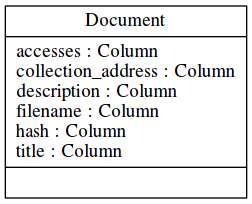
\includegraphics{classes_document.png} 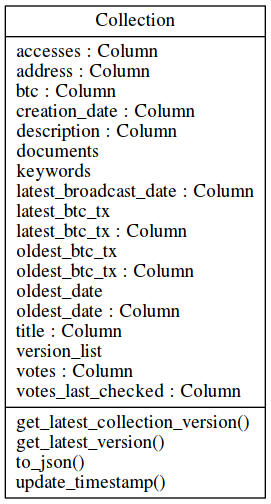
\includegraphics{classes_collection.png} 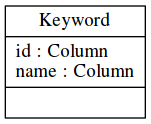
\includegraphics{classes_keyword.png} 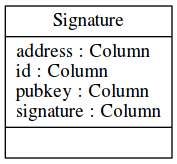
\includegraphics{classes_signature.png}}

\scalebox{.500000}{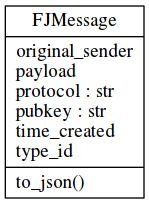
\includegraphics{classes_fj_message.png}}

Each Column is a database column in our local cache.  Each file represents a type
of database table and therefore entry.  These models also form the base classes
for the backend of the freejournal API.

The fj\_message model does not represent a database object, instead serving as the interface
between JSON messages described on the Protocol page and the database representation of the objects in the cache.


\subsection{Cache}
\label{architecture:cache}
\scalebox{.500000}{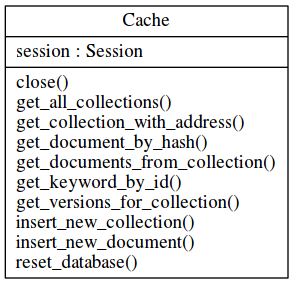
\includegraphics{classes_cache.png}}

\scalebox{.500000}{
\includegraphics{classes_db.png}}

The cache is intended to provide an abstraction for dealing with database objects
such as the models above, simplifying application syntax.  The cache also stores
the current session to allow for session reuse.


\subsection{Controllers}
\label{architecture:controllers}
\scalebox{.500000}{
\includegraphics{classes_collections.png}}
\scalebox{.500000}{\includegraphics{classes_controller.png}}

The controller files provide for an API for packages using the core freejournal
library to manipulate the models.


\subsection{Bitmessage Connection}
\label{architecture:bitmessage-connection}
\scalebox{.500000}{
\includegraphics{classes_bitmessage_keepalive.png}}

\scalebox{.500000}{
\includegraphics{classes_bitmessage_listener.png}}

\scalebox{.500000}{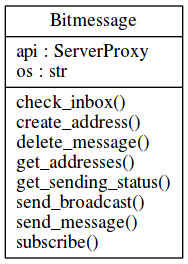
\includegraphics{classes_bitmessage.png}}

\scalebox{.500000}{
\includegraphics{classes_install.png}}

These classes are responsible for communicating with the BitMessage software, which
provides a communication channel over which freejournal nodes communicate with each other.

The listener listens for new messages coming in on the network, dispatching them to be processed
and added to the local cache if necessary.  The connection is also responsible for publishing
new messages to the network, broadcasting collections to the network at large.

The instal class is responsible for preparing dependencies associated with Bitmessage communication.


\subsection{Freenet Connection}
\label{architecture:freenet-connection}
\scalebox{.500000}{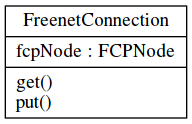
\includegraphics{classes_FreenetConnection.png}}

\scalebox{.500000}{
\includegraphics{classes_install.png}}

The Freenet connection is responsible for communication with the Freenet network, uploading and downloading
the document bodies synchronized in collections over the Bitmessage network.


\subsection{Bitcoin Connection}
\label{architecture:bitcoin-connection}
\scalebox{.500000}{\includegraphics{classes_timestampfile.png}}

The timestamp class is responsible for communicating with the Bitcoin network to both retreive and upload
timestamps for given collection hashes.  The timestamp library currently uses the \href{http://proofofexistence.com/}{ProofOfExistence API}.

\subsection{Sequence Diagrams}
\label{architecture:sequence-diagrams}
The following are the sequence diagrams for the primary use cases implemented in the FreeJournal system,
corresponding to use cases 1-5 on the architecture page (and subsuming several of the remaining use cases).

\emph{Use Case 1} \\
\label{architecture:use-case-1}
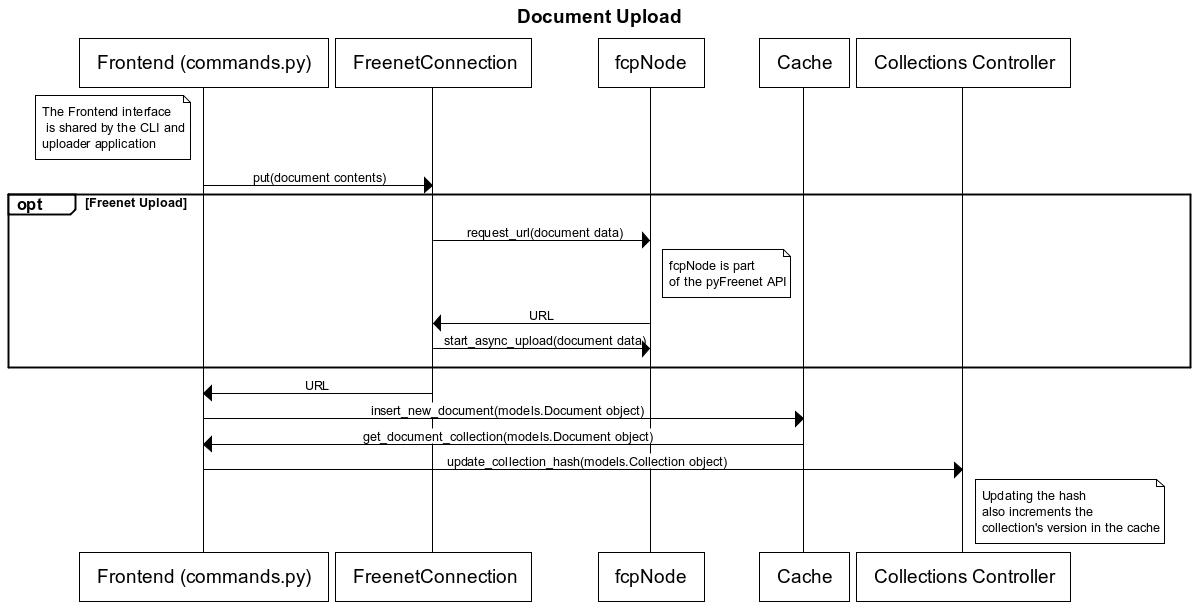
\includegraphics{UC1.png}


\emph{Use Case 2} \\
\label{architecture:use-case-2}
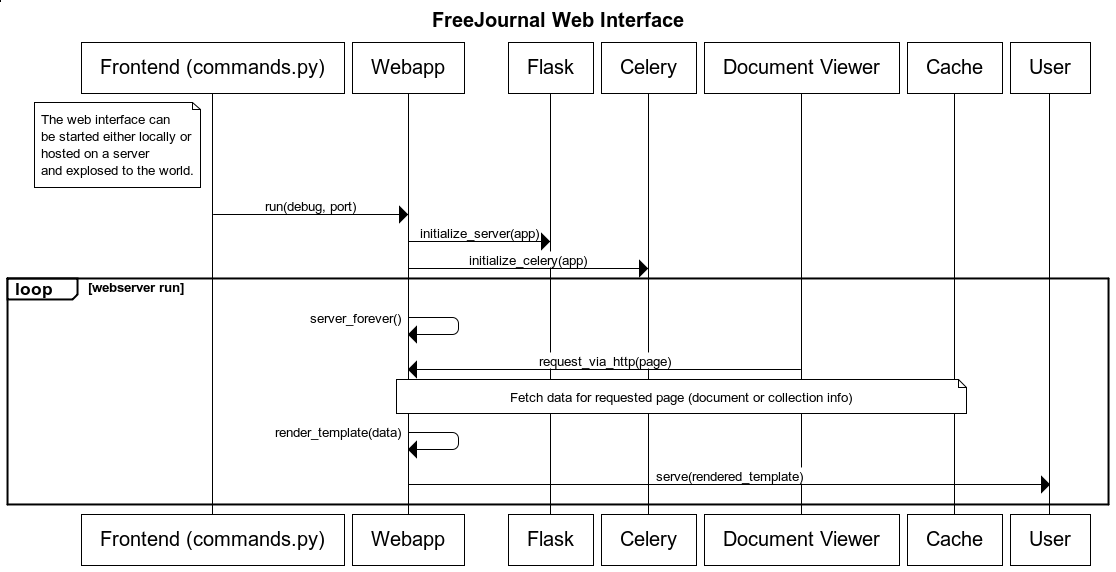
\includegraphics{UC2.png}


\emph{Use Case 3} \\
\label{architecture:use-case-3}
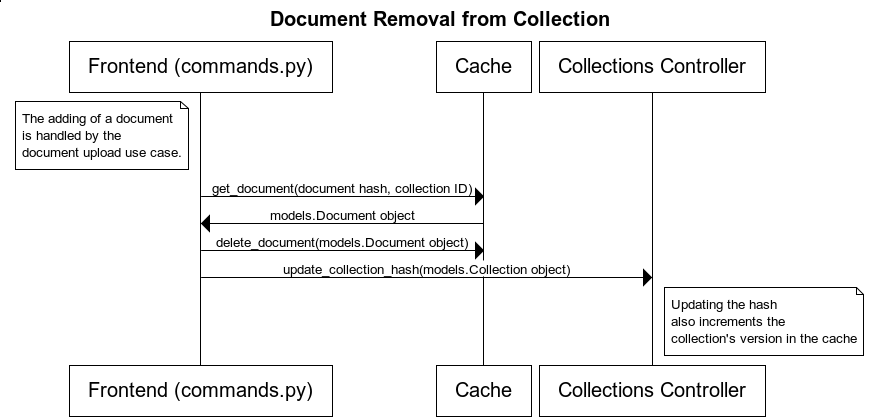
\includegraphics{UC3.png}


\emph{Use Case 4} \\
\label{architecture:use-case-4}
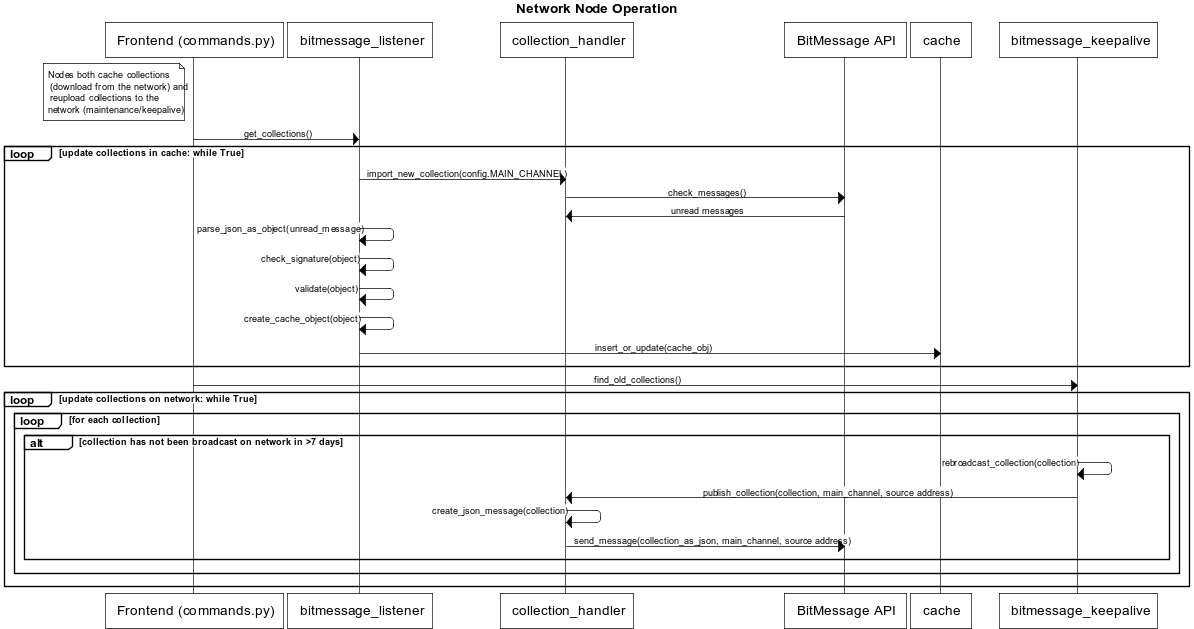
\includegraphics{UC4.png}


\emph{Use Case 5} \\
\label{architecture:use-case-5}
\includegraphics{UC5.png}

\chapter{Future Plans}
\label{future:future-plans}\label{future::doc}
Our future plans include extending the functionality of FreeJournal to that of a complete
document and binary data upload and sharing platform.  The following features still need
improvement or implementation:
\begin{itemize}
\item {} 
Bitcoin timestamping (better frontend integration)

\item {} 
Bitcoin voting / ranking algorithms

\item {} 
Robustness / scalability tests with large datasets

\end{itemize}


\section{Team Member Reflections}
\label{future:team-member-reflections}
in no particular order.


\subsection{Dan}
\label{future:dan}
Overall I had a great time working on this project and learned a good deal. I really liked the concept and
goals of the project. I worked mostly on backend of the project with integrating a couple dependencies to help
achieve our goals. In terms of process I had a good time working with everyone in our group and belive we
functioned very well to complete it.

The scrum development process worked well for us as it was flexible and easy to follow. What I learned most
during the project was about the benefits and headaches of depending on so many different libraries/softwares.
Our project probably isn't possible without things like FreeNet and Bitmessage, however the source of most
problems came from these dependencies.


\subsection{Wenxue}
\label{future:wenxue}
I am working on the back-end. It is a good experience to work on a project from ideation to research, design,
and development. We are using a lot of libraries, such as Bitcoin blockchain, Bitmessage, Freenet and etc. One
of the issues I am working on is using Bitcoin transactions timestamp the documentation. When I was working on
it, I learned how to do some research on the new concepts I did not know before and use them in the project.


\subsection{Walker}
\label{future:walker}
Working on this project was a productive learning experience. It was a great chance to develop my skills
working with Git and Python, and was the first chance I've had to work on a larger-scale project using GitHub.
Our implementation of Scrum, which used GitHub's issue system to keep track of tickets, seemed to work pretty
well, especially given our weekly pace for meetings. My role was primarily focused on the front-end website.
It was implemented using Flask, which allowed us to easily integrate the web server with the FreeJournal
command line interface. Additionally, I worked on integrating SQLAlchemy and the caching system that stores
documents locally, as well as the Bitmessage listener routine. Initially I suggested to the group that we use
Celery to create asynchronous jobs and repeating tasks, but it ended up being too heavy of a dependency to
include and instead I ended up implementing the repeating tasks using Python’s threading APIs.


\subsection{Brian}
\label{future:brian}
Going into choosing a project team, I was determined to find a project that reflected my ideals, challenged me
technologically, and ultimately was something that I was proud to put on my resume and show employers what I
could accomplish in a full year long project. After reflecting on the project from beginning to end, I
couldn’t be happier I chose Freejournal. I worked mostly on the Freenet side of the project, focusing on
handling the submission and retrieval of ‘documents’ that have been leaked onto the freejournal network. As
the project went on, I quickly discovered the integration that the project required a complete knowledge of
the architecture, in order to fully understand what was happening at any given time. I feel like one of the
most challenging parts of this project was understanding how all the dependencies fit together to create a
finished project. This was largely realized in the complexity of our UML diagrams. Realizing just how
complicated the stream of execution was on more complicated projects almost necessitates the visualization of
some sort of stream of execution. This is what separates a “coder” from a “software engineer”, and why the
latter is so important to software projects.


\subsection{Fernando}
\label{future:fernando}
Working with a team on the Free Journal project has been a blast! I worked on the file timestamp module as
well as the GUI for the document uploader. I learned a lot from the ideas and skills of my teammates.
Especially that software bugs can appear when you least expect them. Everyone had something different to
contribute and the Scrum method helped leverage that quality. As a result, we achieved our objectives and
gained valuable experience working together as a team.


\subsection{Phil}
\label{future:phil}
I had a great time with all the guys on the team, and would definitely say it was a cohesive, informative,
and fun learning experience.  My primary role was organizational, focusing on developing the core ideas of
the project through documentation, code review, process management, and other specification creation.  I
was responsible for the documentation and creation of the Protocol Specification.  In additon, I also worked
on several refactorings, unit test additions, repository reorganizations, and other maintenance tasks.  Lastly,
I co-developed the initial models / cache architecture.  I really think the Scrum process and the Github-style
development we describe in this document was a great fit for our team, and I was surprised by how robust and
usable our final project is considering its complexity.  Overall, we didn't finish everything we set out to do,
but we still managed to put out an impressive piece of peer to peer software in a single semester... so I call
that a big win!


\subsection{Drew}
\label{future:drew}
It was interesting to work on a somewhat large project from start to finish with seven people.  I believe the
scrum process and our branch organization on Github allowed for consistent progress towards our goals.  A take
away for this project is to have all the merging for a development cycle done and tested at least a couple
days before the deadline.  Other than that, I think the project went smoothly.



\renewcommand{\indexname}{Index}
\printindex
\end{document}
